\documentclass[12pt, a4]{report}
    \usepackage[utf8]{inputenc}
    \usepackage[croatian]{babel}
    \usepackage{graphicx}
    \usepackage[a4paper, total={6in, 10in}]{geometry}
    \usepackage{caption}
    \usepackage{amsmath}
    \usepackage{subfig}

    \graphicspath{ {res/} }

    \title{Laboratorijska vježba 2}
    \author{Matija Marić, 0036479678}
    \date{\today}

    \begin{document}
        \begin{titlepage}
            \maketitle
        \end{titlepage}

        \tableofcontents{}

        \chapter{Frekvencijske transformacije}
        \section{Diskretna Fourierova transformacija}
            \begin{enumerate}
                \item
                    \begin{minipage}{\linewidth}
                        \centering
                        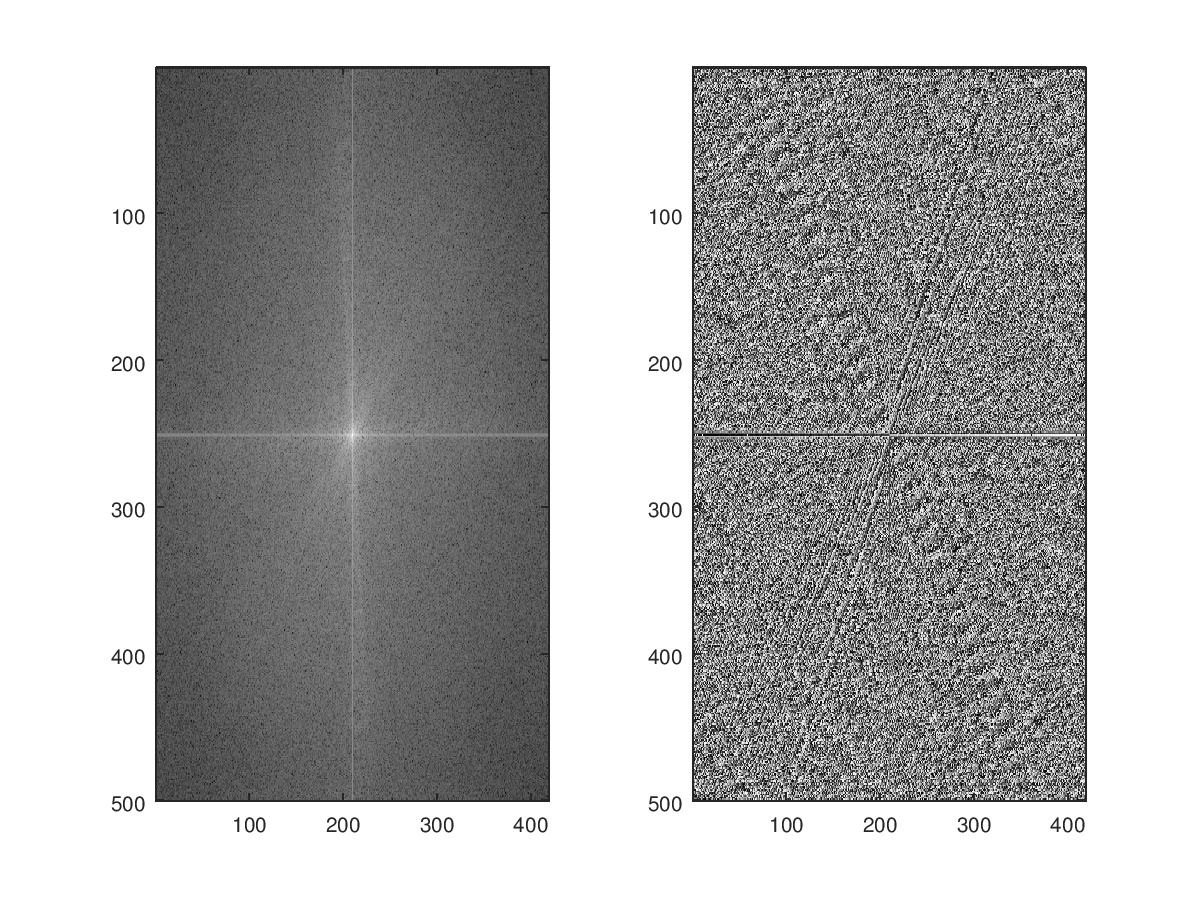
\includegraphics[width=0.75\textwidth]{fft1}
                        \captionof{figure}{Spektar slike {\it klis2.png}}
                    \end{minipage}
                    \begin{minipage}{\linewidth}
                        \centering
                        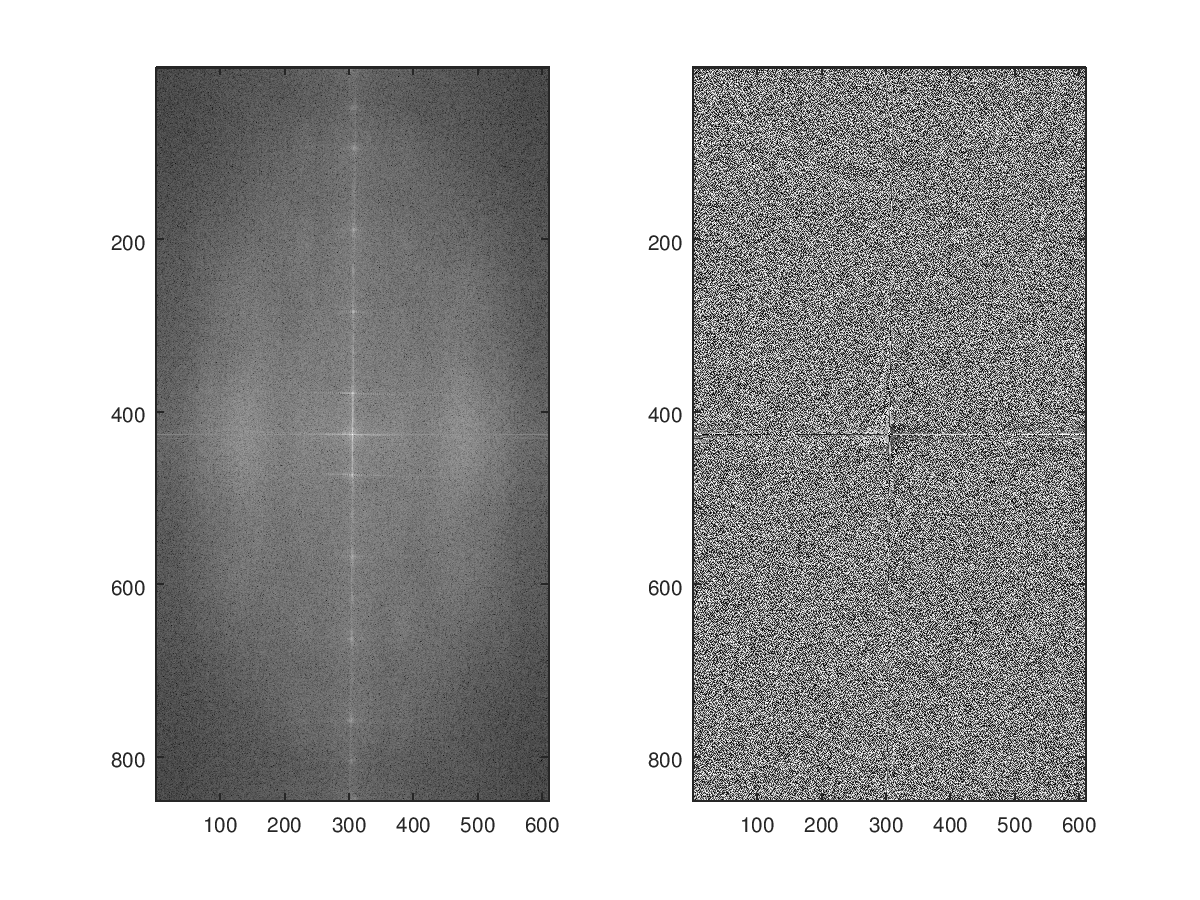
\includegraphics[width=0.75\textwidth]{fft2}
                        \captionof{figure}{Spektar slike {\it misal\_1483.png}}
                    \end{minipage}
            \end{enumerate}
        
        \section{DFT i geometrijske transformacije slike}
            \begin{enumerate}
                \item
                    \begin{minipage}{\linewidth}
                        \centering
                        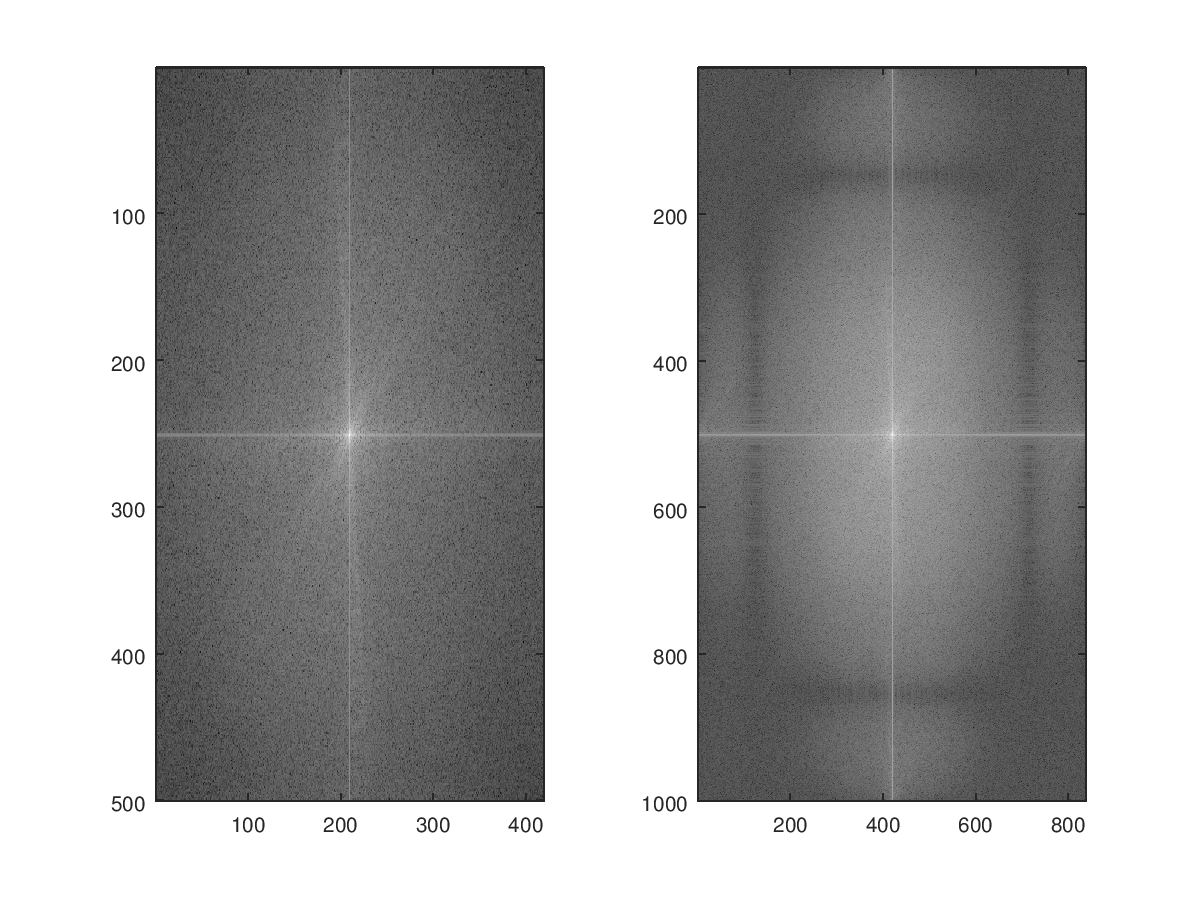
\includegraphics[width=0.75\textwidth]{klis_scaled}
                        \captionof{figure}{Amplitudni spektri originalne i skalirane slike {\it klis2.png}}
                    \end{minipage}
                    Skalirani spektar se periodički ponavlja.
                \item
                    \begin{minipage}{\linewidth}
                        \centering
                        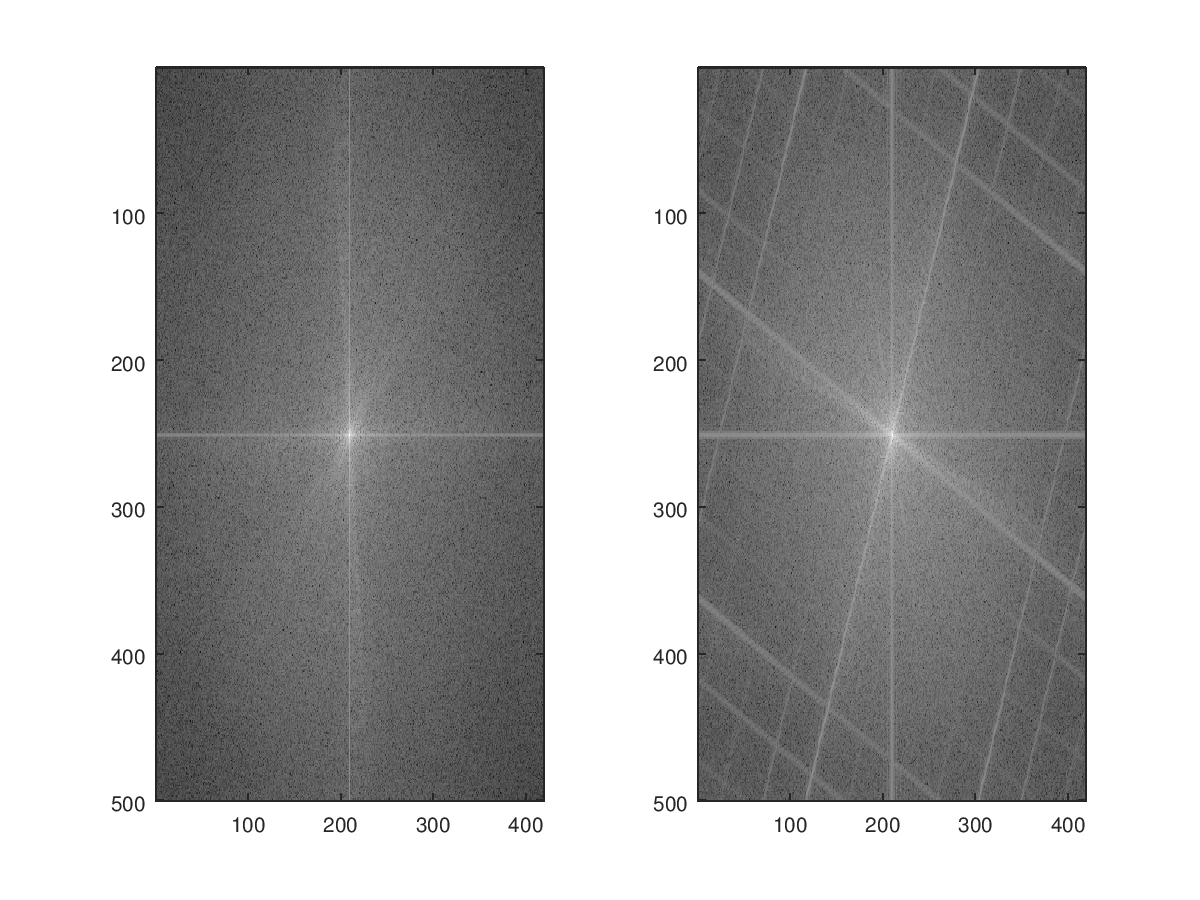
\includegraphics[width=0.75\textwidth]{klis_rotated}
                        \captionof{figure}{Amplitudni spektri originalne i rotirane slike {\it klis2.png}}
                    \end{minipage}
                    Spektar rotirane slike je isto rotiran.
                \item
                    \begin{minipage}{\linewidth}
                        \centering
                        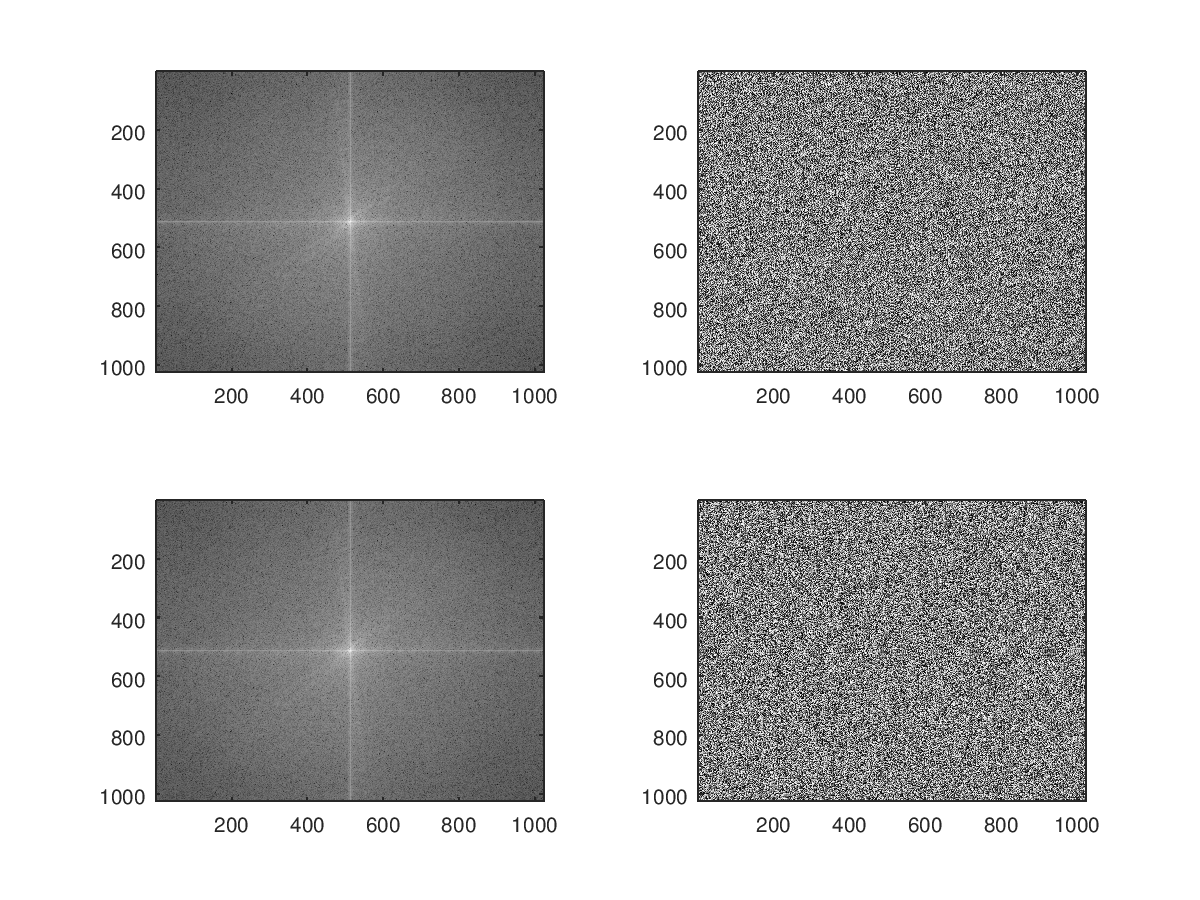
\includegraphics[width=0.75\textwidth]{klis_translated}
                        \captionof{figure}{Spektri originalne i translatirane slike {\it klis2.png}}
                    \end{minipage}
                \item
                    Ne vidi se ništa jasno iz faznog spektra slika.
            \end{enumerate}
        \section{Filtriranje slike}
            \begin{enumerate}
                \item
                    \begin{minipage}{\linewidth}
                        \centering
                        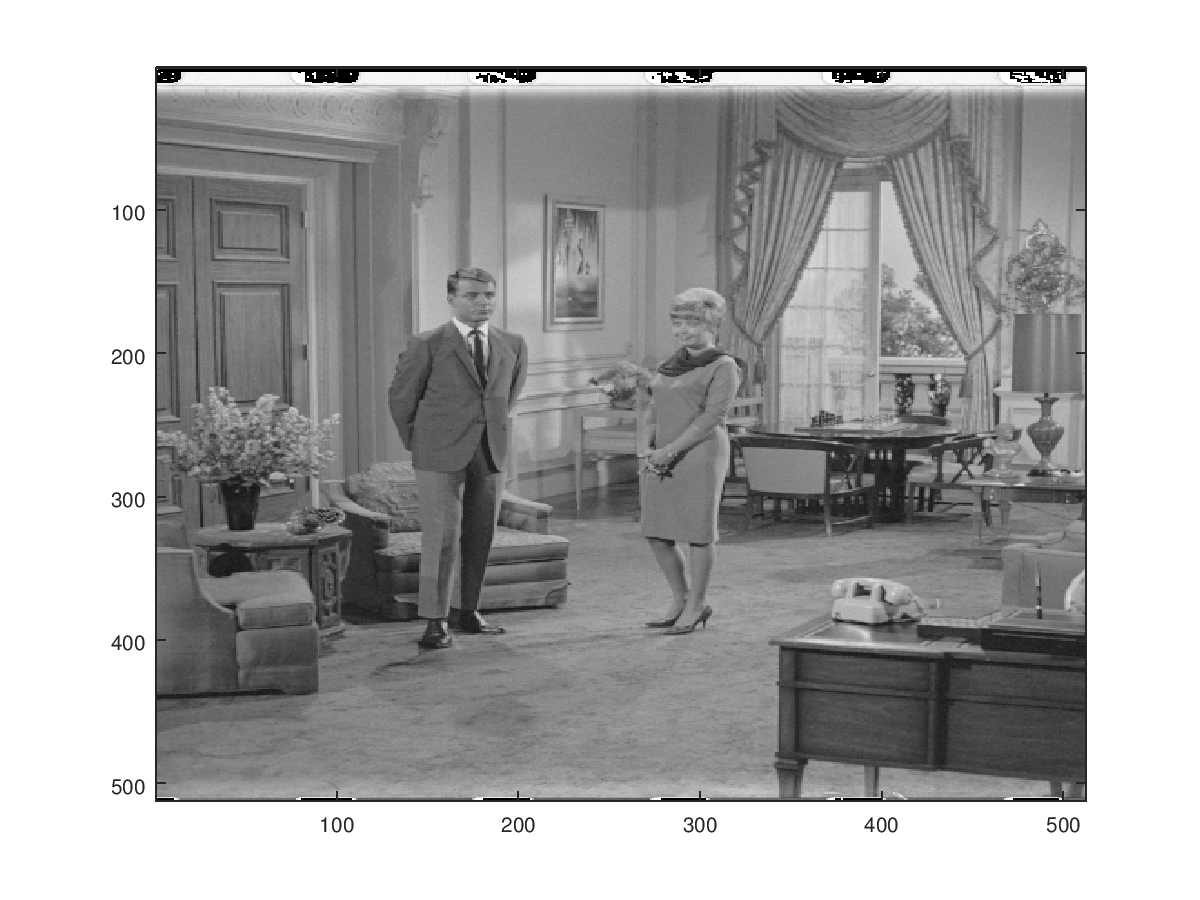
\includegraphics[width=0.75\textwidth]{couple}
                        \captionof{figure}{Originalna slika {\it couple.tiff}}
                    \end{minipage}
                    \begin{minipage}{\linewidth}
                        \centering
                        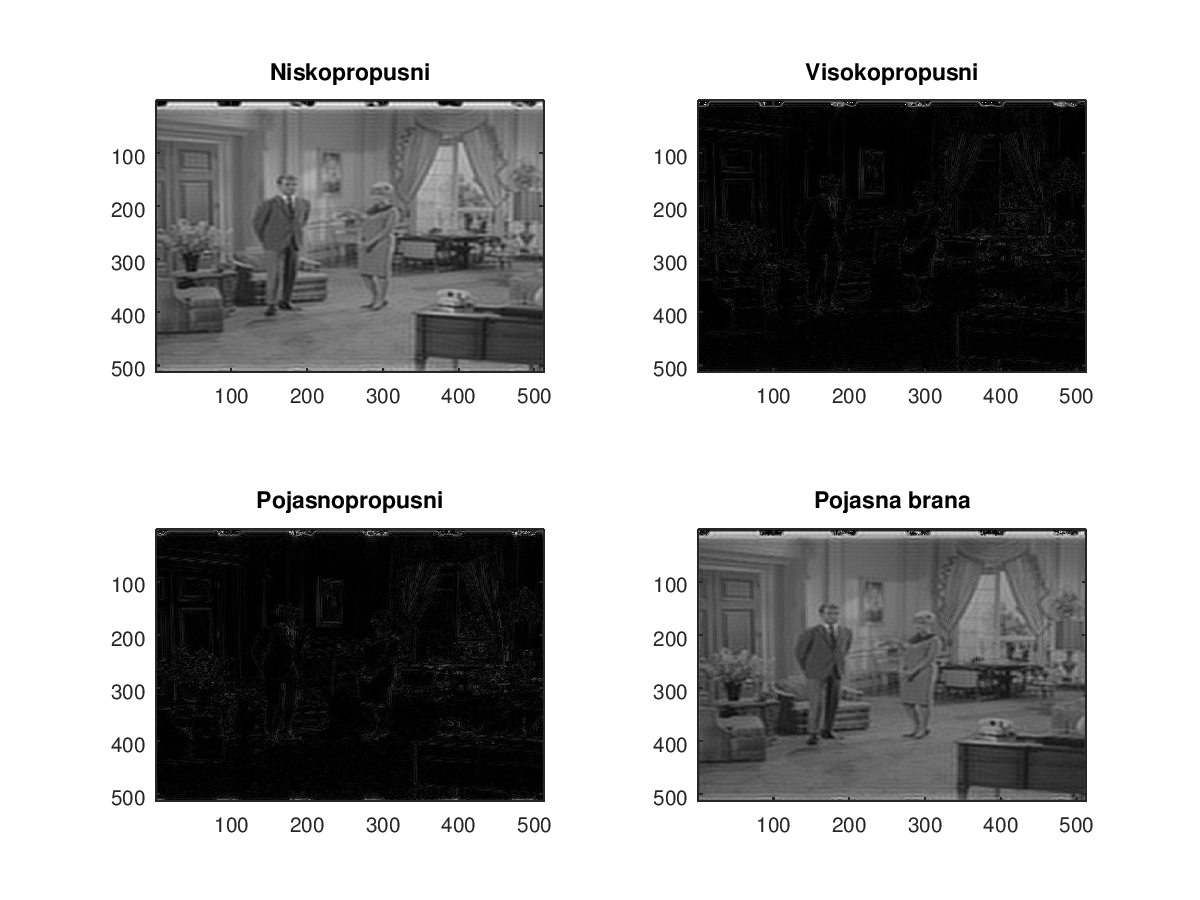
\includegraphics[width=0.75\textwidth]{filteri}
                        \captionof{figure}{Slika {\it couple.tiff} sa svim vrstama frekvencijskih filtera.}
                    \end{minipage}
                
            \end{enumerate}
        \section{Diskretna kosinusna transformacija}
            \begin{enumerate}
                \item
                    \begin{minipage}{\linewidth}
                        \centering
                        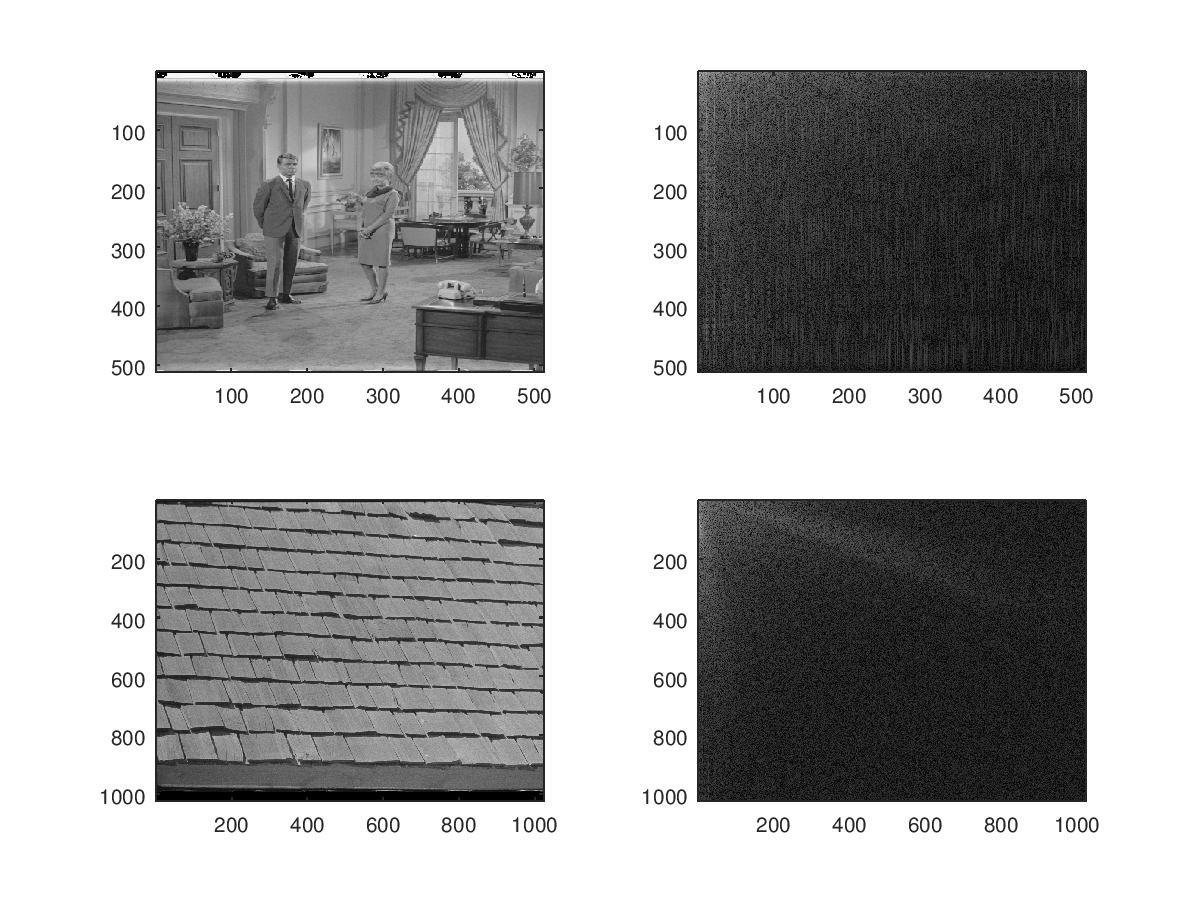
\includegraphics[width=0.75\textwidth]{cosine}
                        \captionof{figure}{Slike {\it couple.tiff} i {\it roof.tiff} i njihove diskretne kosinusne transformacije.}
                    \end{minipage}
                \item
                    Istosmjerna komponenta se nalazi i gornjem lijevom kutu spektra.
                \item
                    Kod DCT je više energije u niskofrekvencijskom dijelu spektra.
            \end{enumerate}
        \section{DCT i kompresija slike}
            \begin{enumerate}
                \item
                    \begin{minipage}{\linewidth}
                        \centering
                        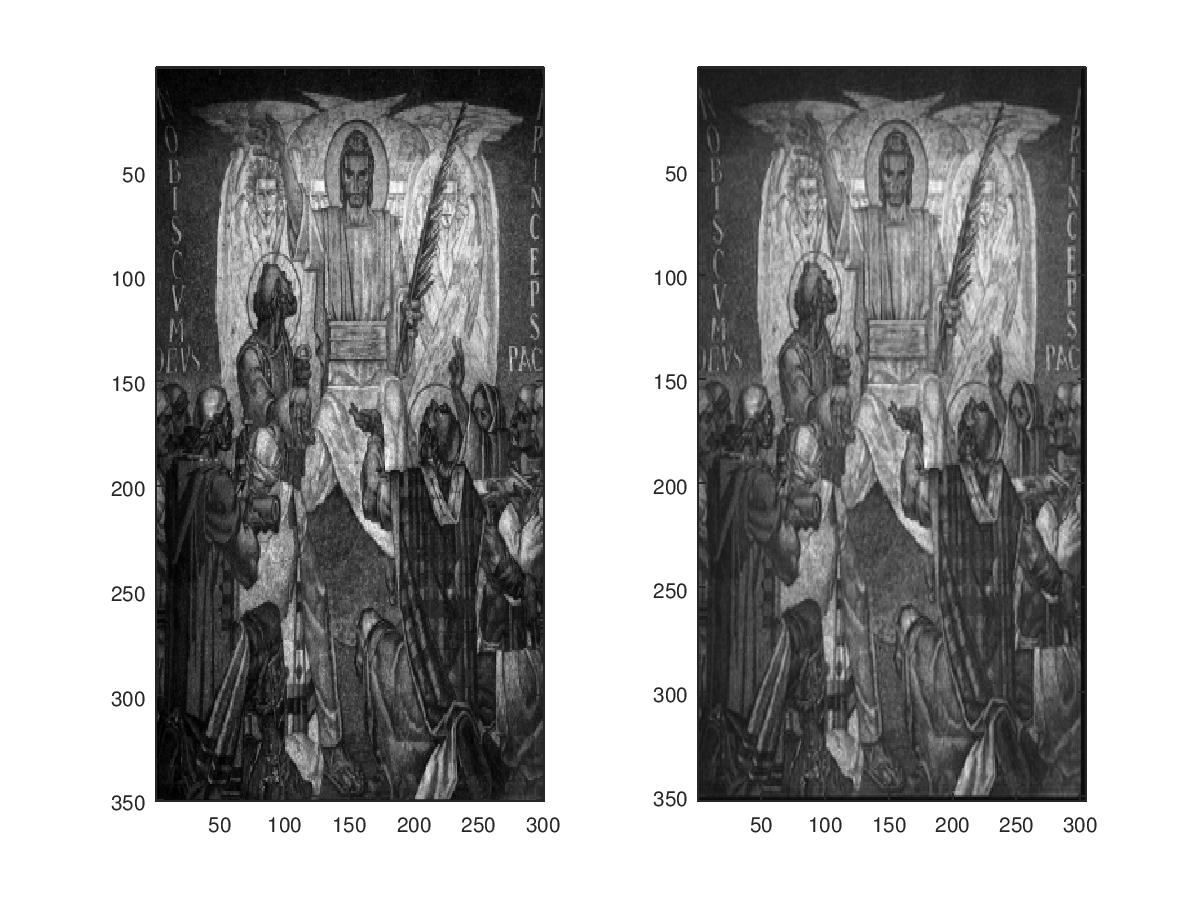
\includegraphics[width=0.75\textwidth]{dct_compression}
                        \captionof{figure}{Originalna i kompresirana slika {\it kljakovic2.png}. Korištena je $8\times8$ restrikcijska matrica sa kvadratom $6\times6$.}
                    \end{minipage}
                \item
                    Srednja kvadratna greška je 22.848.
                \item
                    Povećanjem maske povećavamo kvalitetu slike i smanjujemo kvadratnu grešku. Trokutasta maska ima veću grešku od kvadratne maske istih dimenzija.
                \item
                    \begin{minipage}{\linewidth}
                        \centering
                        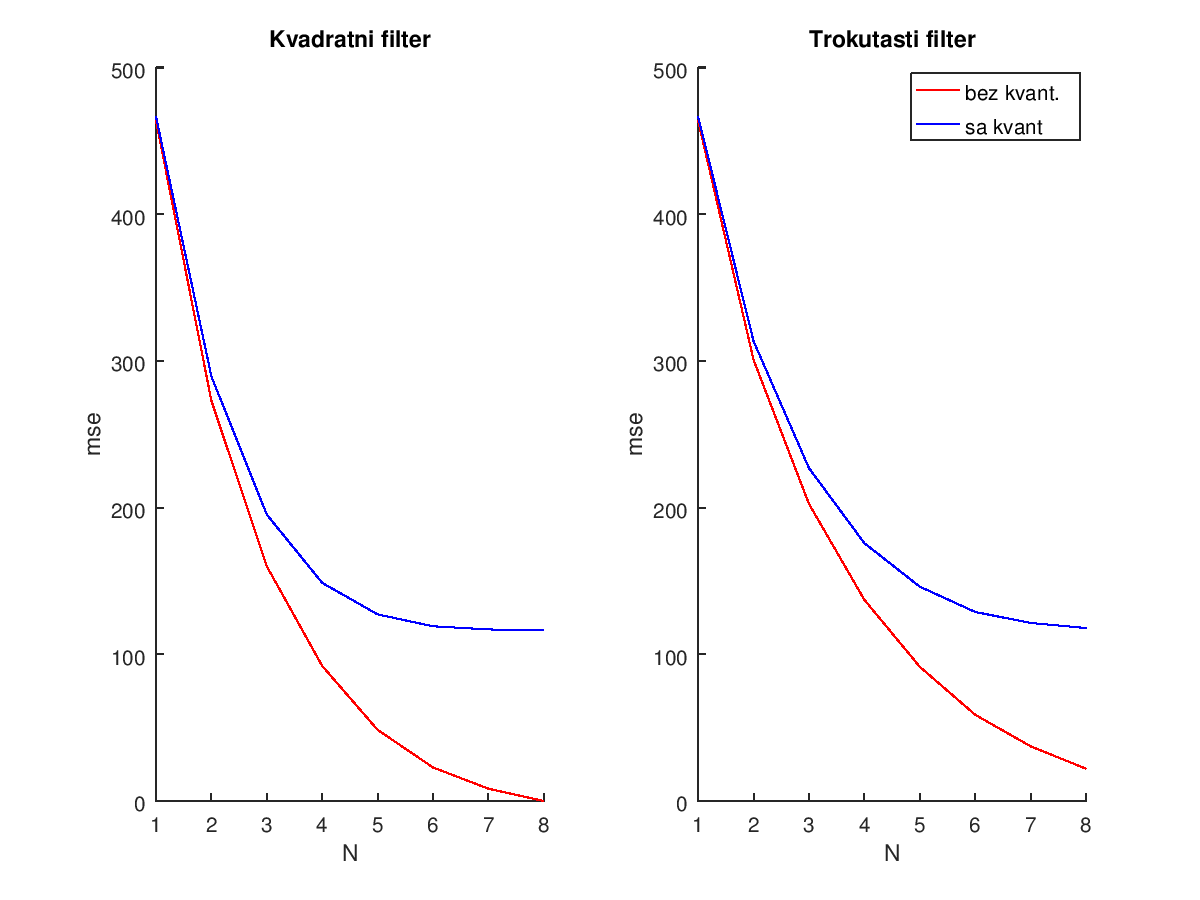
\includegraphics[width=0.75\textwidth]{mse_plots}
                        \captionof{figure}{Srednja kvadratna greška za različite parametre maski. Kod kvantizacije je greška neznatno viša.}
                    \end{minipage}
            \end{enumerate}
        
        \chapter{Poboljšanje slike}
        \section{Histogram prvog reda}
            \begin{enumerate}
                \item
                    \begin{minipage}{\linewidth}
                        \centering
                        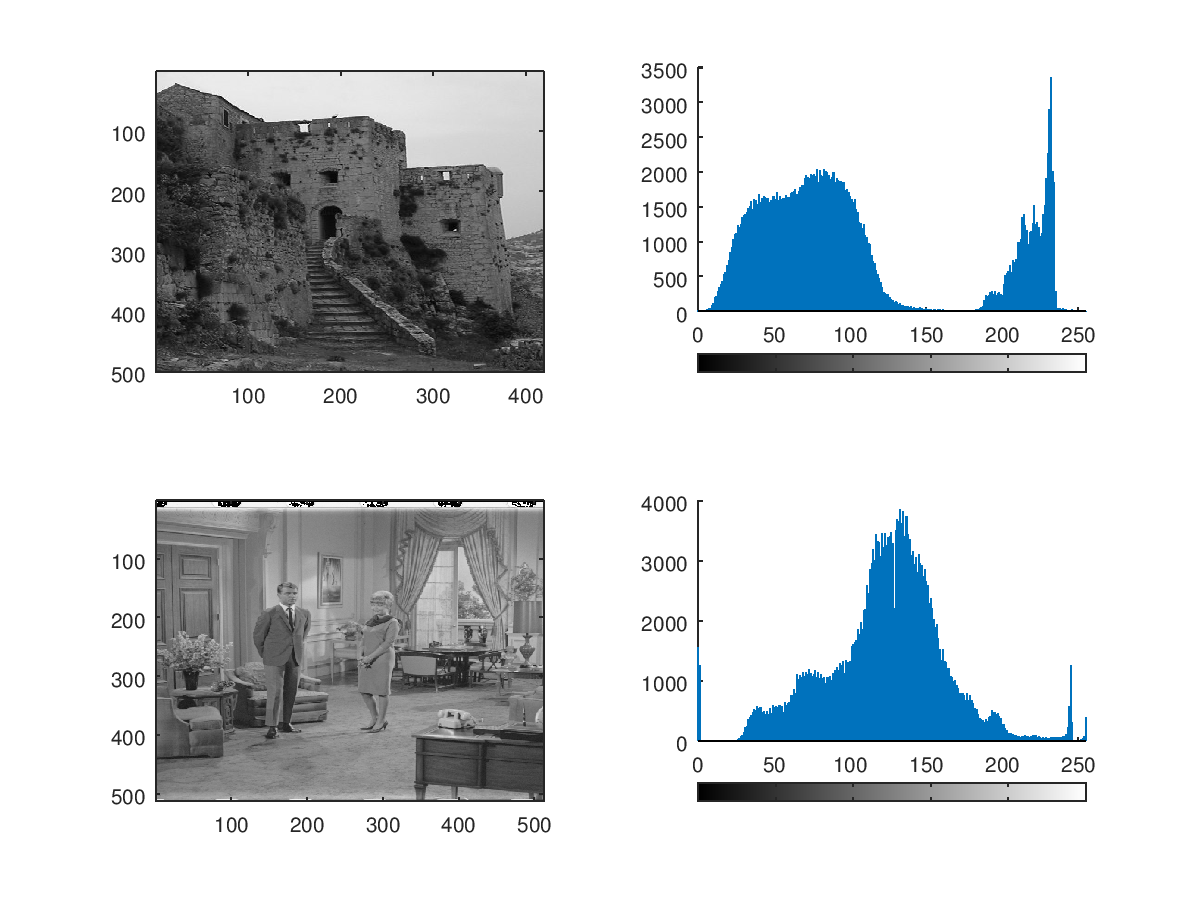
\includegraphics[width=0.75\textwidth]{histograms}
                        \captionof{figure}{Histogrami slika {\it klis.png} i {\it couple.tiff}. X os su razine sive, a y je njihova frekvencija u slici.}
                    \end{minipage} 
            \end{enumerate}
        \section{Izjednačavanje histograma}
            \begin{enumerate}
                \item
                    \begin{minipage}{\linewidth}
                        \centering
                        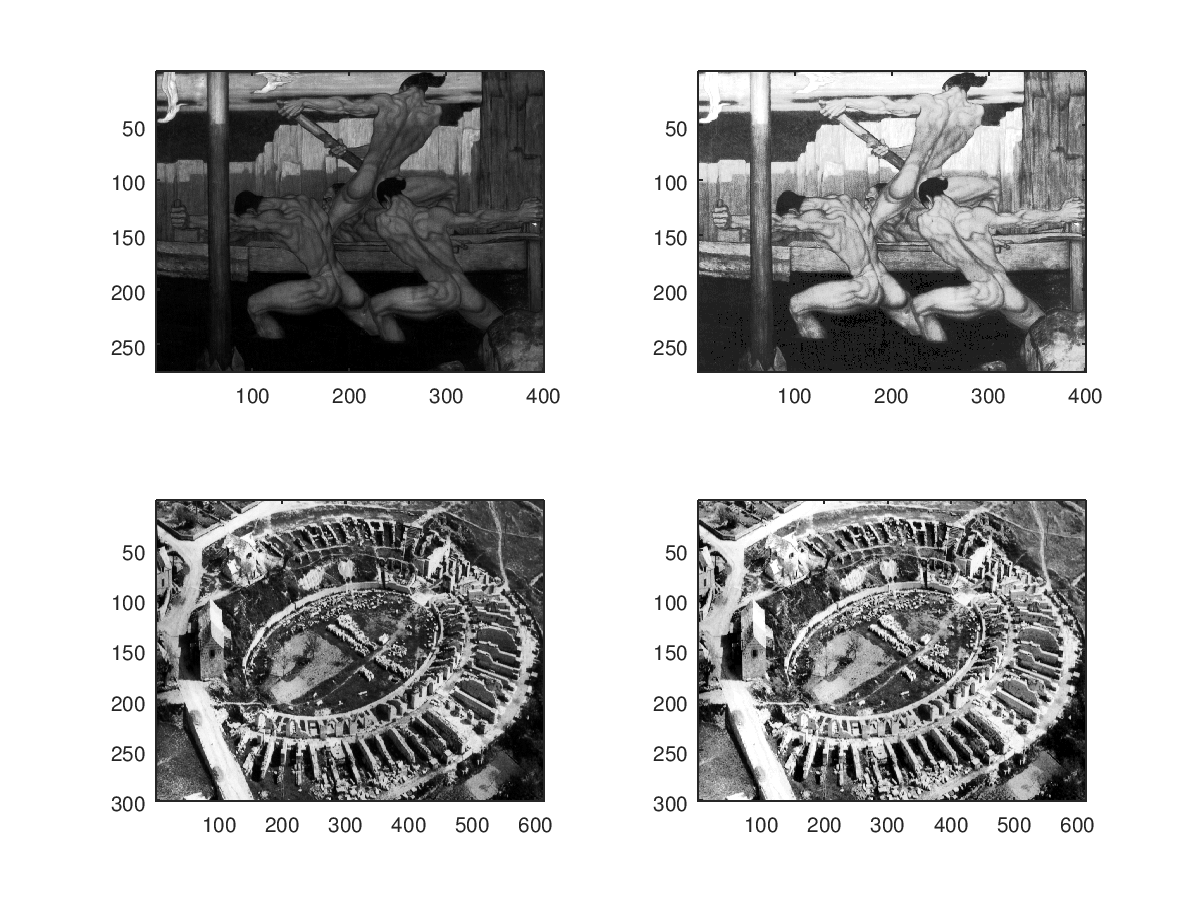
\includegraphics[width=0.75\textwidth]{equalized}
                        \captionof{figure}{Slike {\it uskoci1.png} i {\it salona.png} poboljšane izjednačavanjem histograma.}
                    \end{minipage}
                    \begin{minipage}{\linewidth}
                        \centering
                        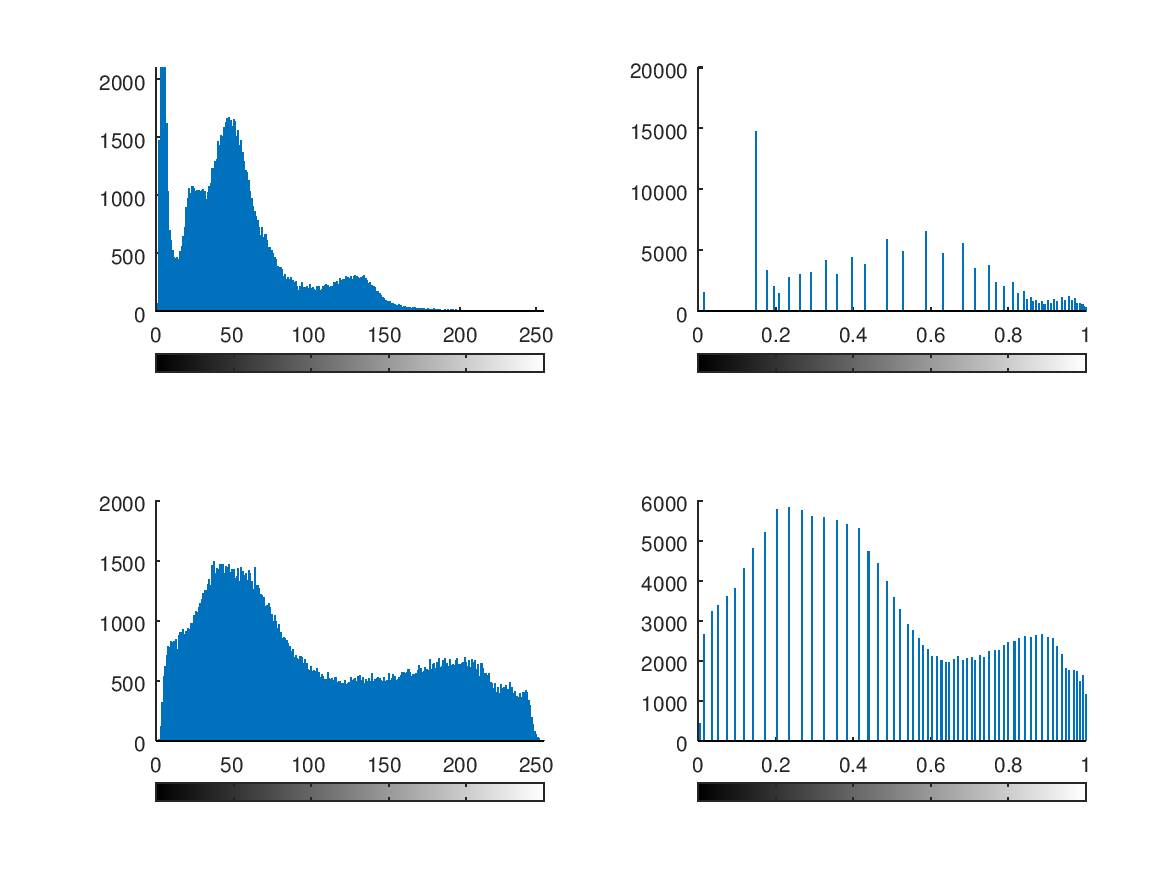
\includegraphics[width=0.75\textwidth]{equalized_histograms}
                        \captionof{figure}{Histogrami slika {\it uskoci1.png} i {\it salona.png} prije i poslije izjednačavanja.}
                    \end{minipage}
                \item
                    Više detalja se vidi nakon izjednačavanja histograma.
            \end{enumerate}
        \section{Modeliranje histograma}
            \begin{enumerate}
                \item
                    \begin{minipage}{\linewidth}
                        \centering
                        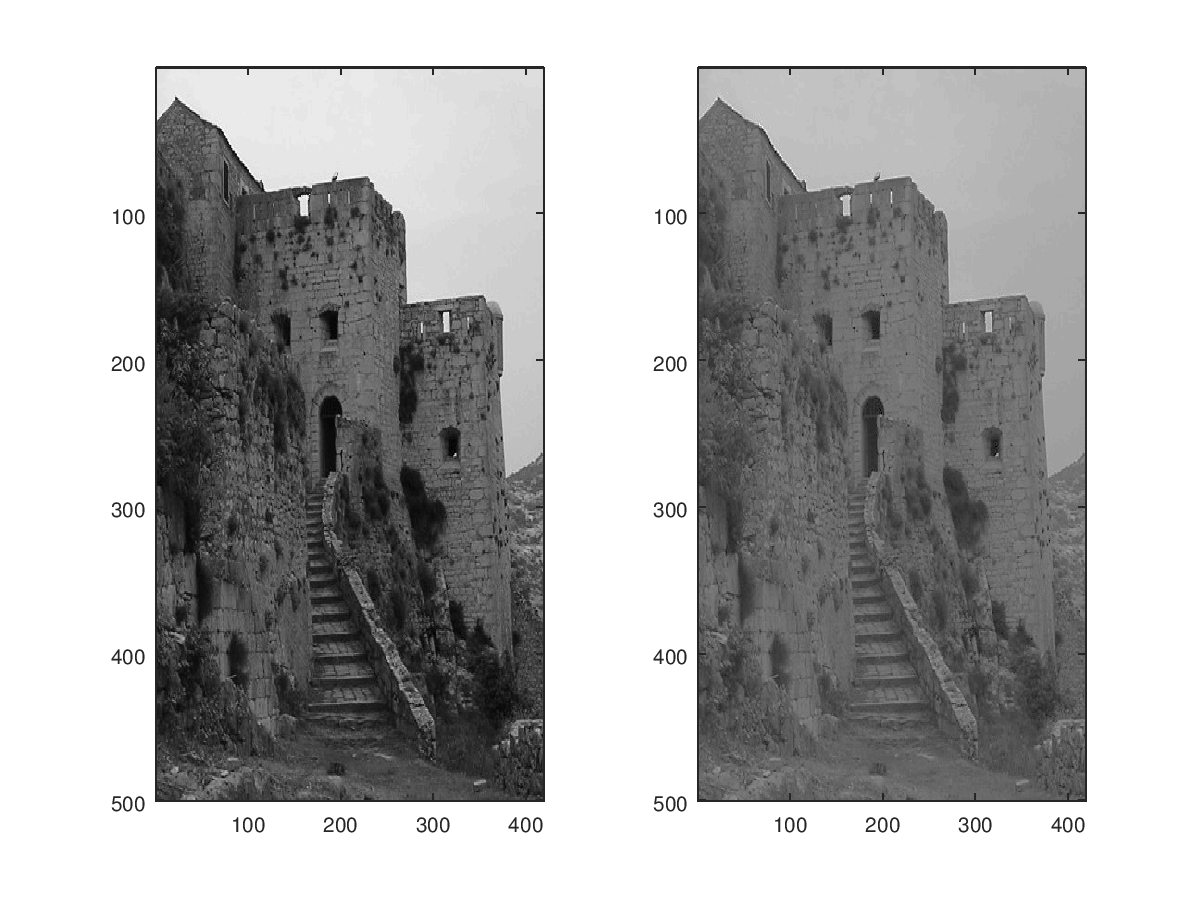
\includegraphics[width=0.75\textwidth]{klis_model}
                        \captionof{figure}{Slika {\it klis2.png} prije i poslije modeliranja.}
                    \end{minipage}
                    \begin{minipage}{\linewidth}
                        \centering
                        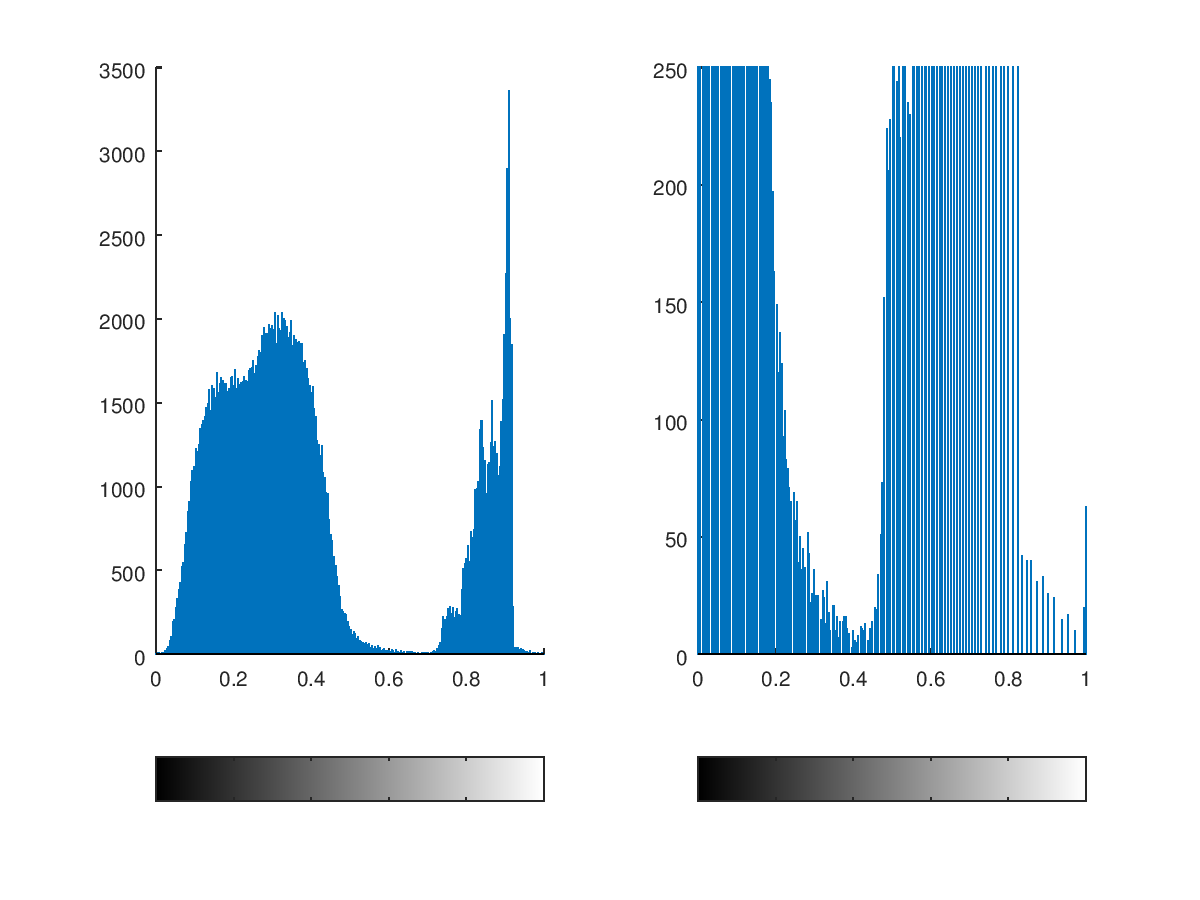
\includegraphics[width=0.75\textwidth]{klis_model_hist}
                        \captionof{figure}{Histogrami slike {\it klis2.png} prije i poslije modeliranja.}
                    \end{minipage}
                \item    
                    \begin{minipage}{\linewidth}
                        \centering
                        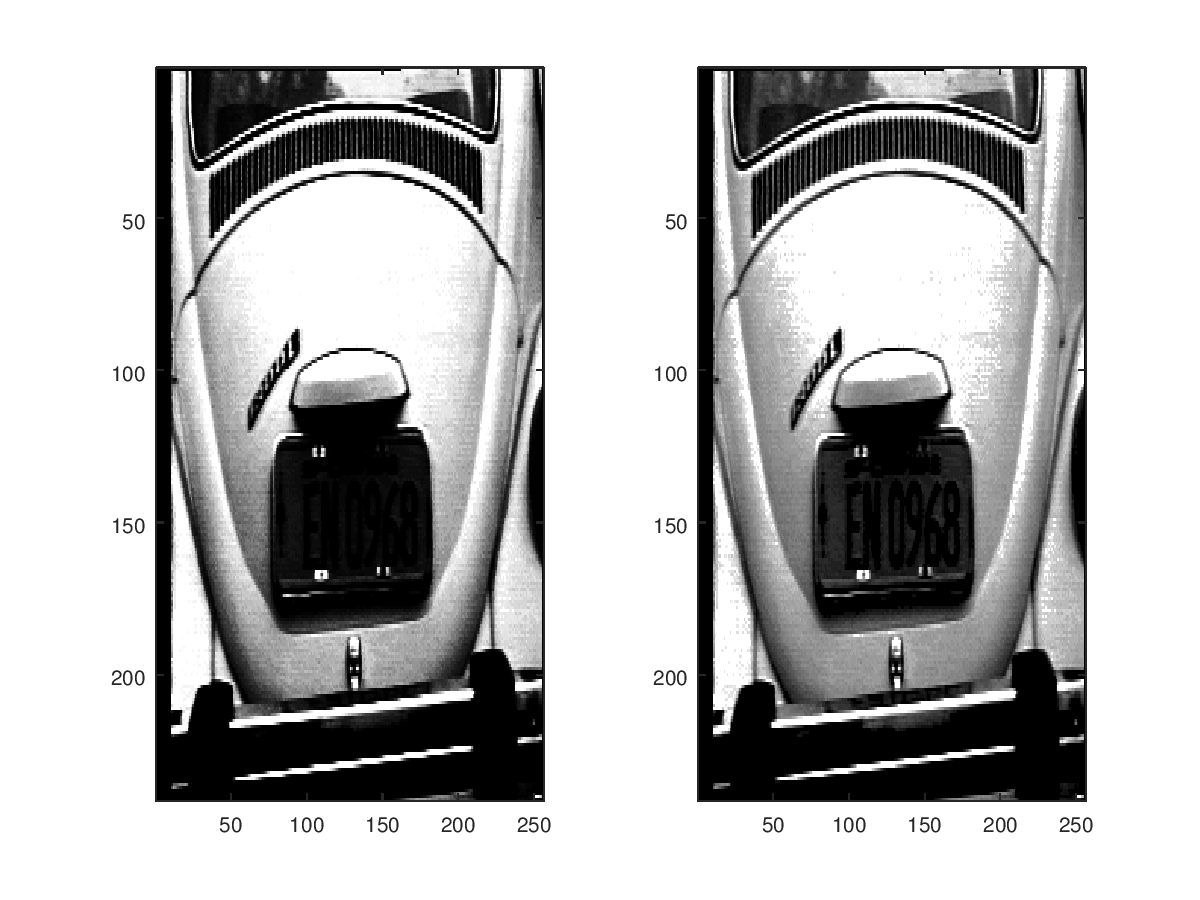
\includegraphics[width=0.75\textwidth]{registracija}
                        \captionof{figure}{Slika registarske tablice poboljšana modeliranjem histograma.}
                    \end{minipage}
            \end{enumerate}
        \section{Usrednjavanje i median filtar}
            \begin{enumerate}
                \item
                    \begin{minipage}{\linewidth}
                        \centering
                        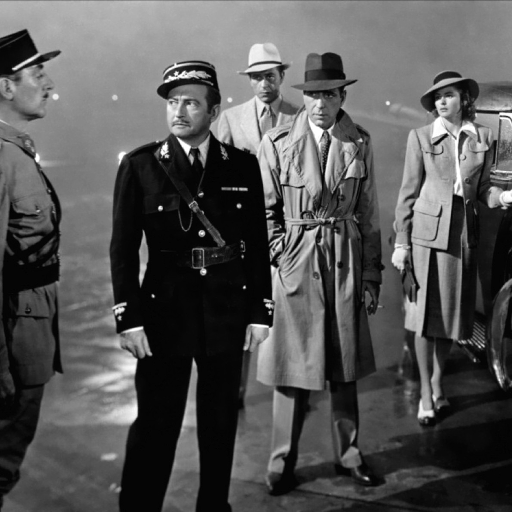
\includegraphics[width=0.75\textwidth]{casablanca}
                        \captionof{figure}{Originalna slika {\it casablanca.png}}
                    \end{minipage}
                    \begin{minipage}{\linewidth}
                        \centering
                        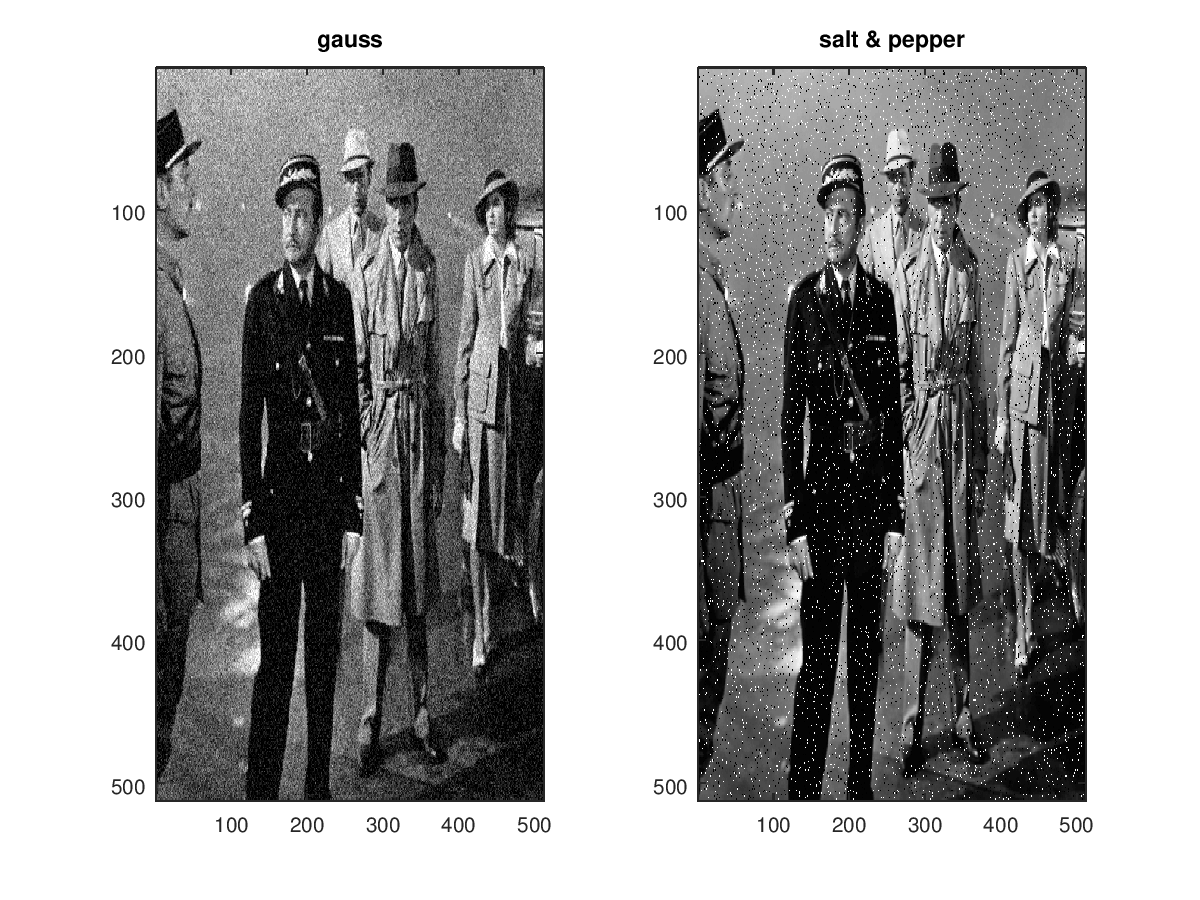
\includegraphics[width=0.75\textwidth]{noise}
                        \captionof{figure}{Slika {\it casablanca.png} sa Gaussovim i impulsnim šumom.}
                    \end{minipage}
                \item
                    \begin{minipage}{\linewidth}
                        \centering
                        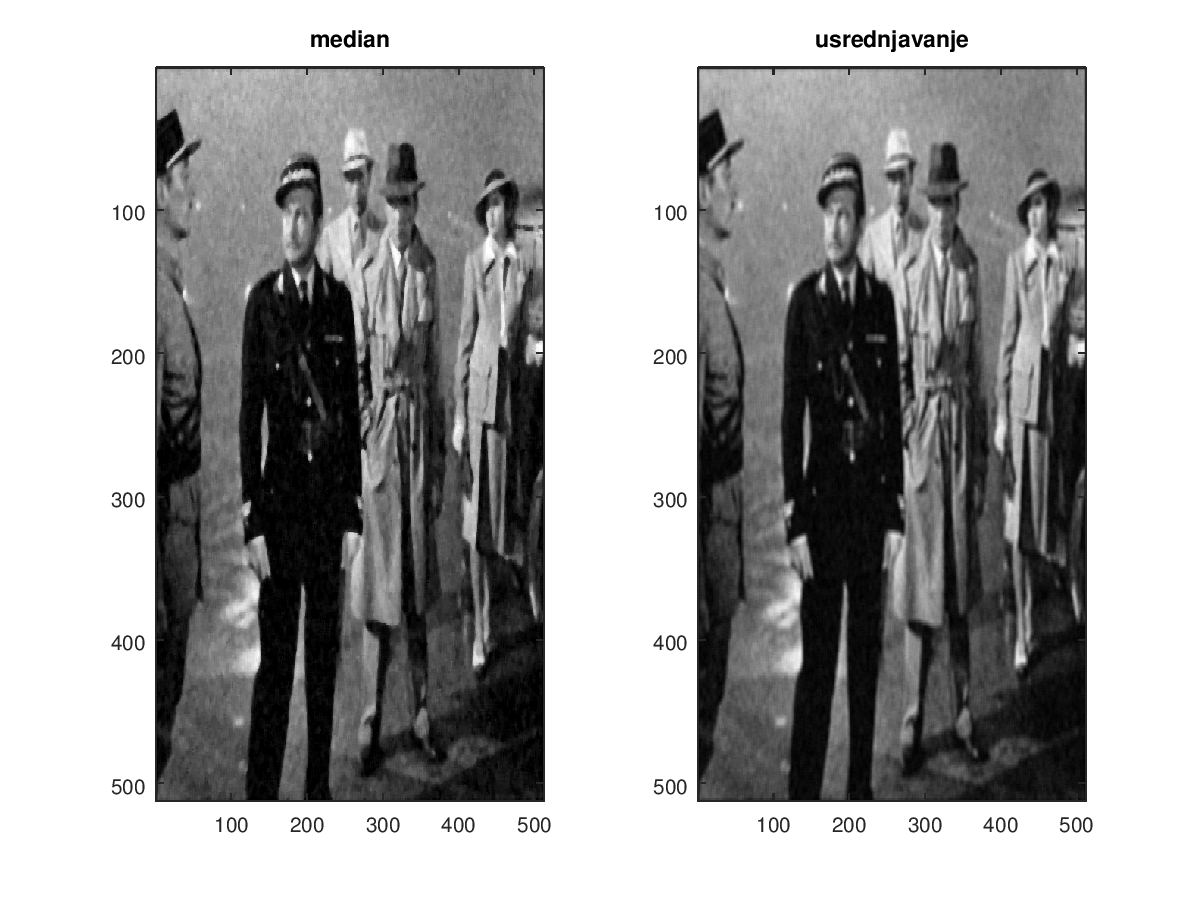
\includegraphics[width=0.75\textwidth]{noise_gauss}
                        \captionof{figure}{Uklanjanje Gaussovog šuma median filterom i usrednjavanjem. Usrednjavanjem se dobivaju bolji rezultati.}
                    \end{minipage}
                    \begin{minipage}{\linewidth}
                        \centering
                        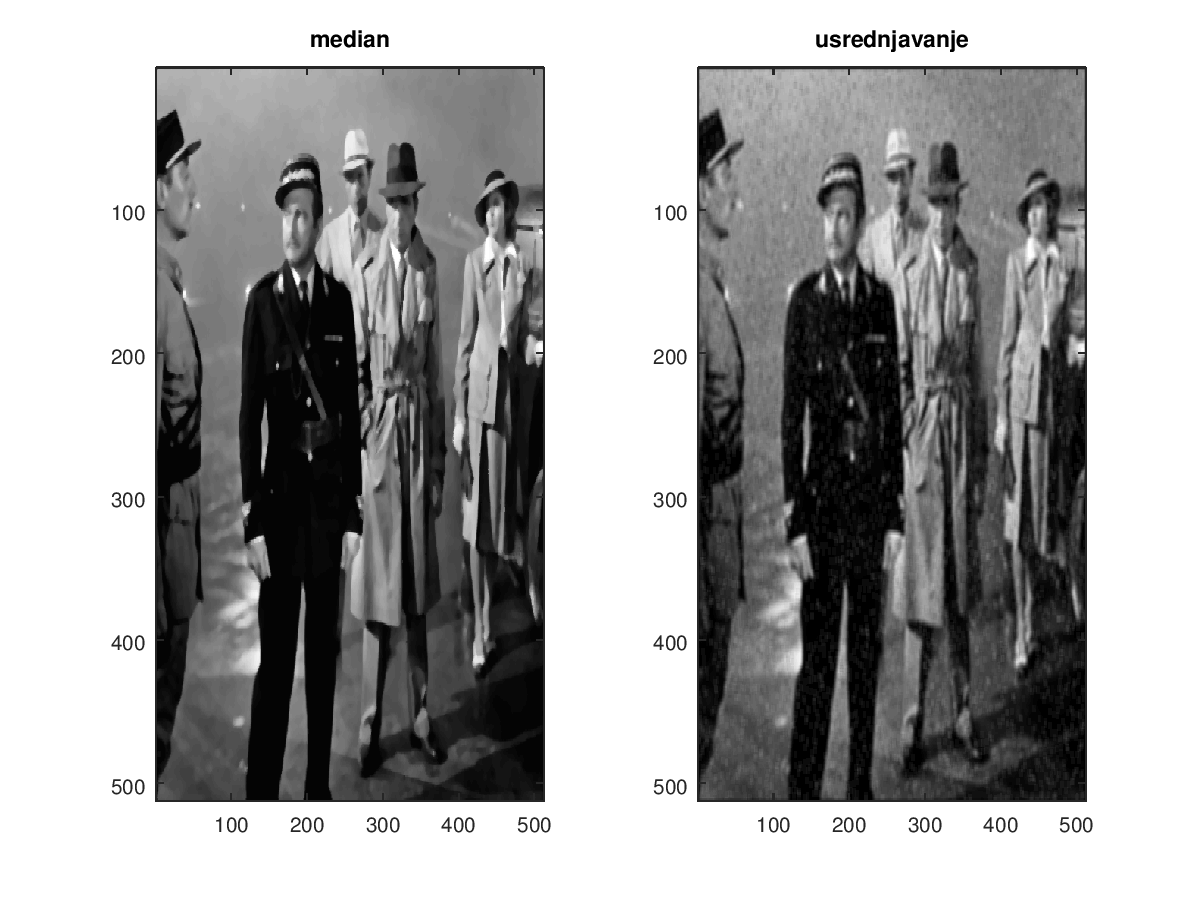
\includegraphics[width=0.75\textwidth]{noise_snp}
                        \captionof{figure}{Uklanjanje impulsnog šuma median filterom i usrednjavanjem. Median filterom se dobivaju bolji rezultati.}
                    \end{minipage}
            \end{enumerate}
        \section{Uklanjanje neoštrine}
            \begin{enumerate}
                \item
                    \begin{minipage}{\linewidth}
                        \centering
                        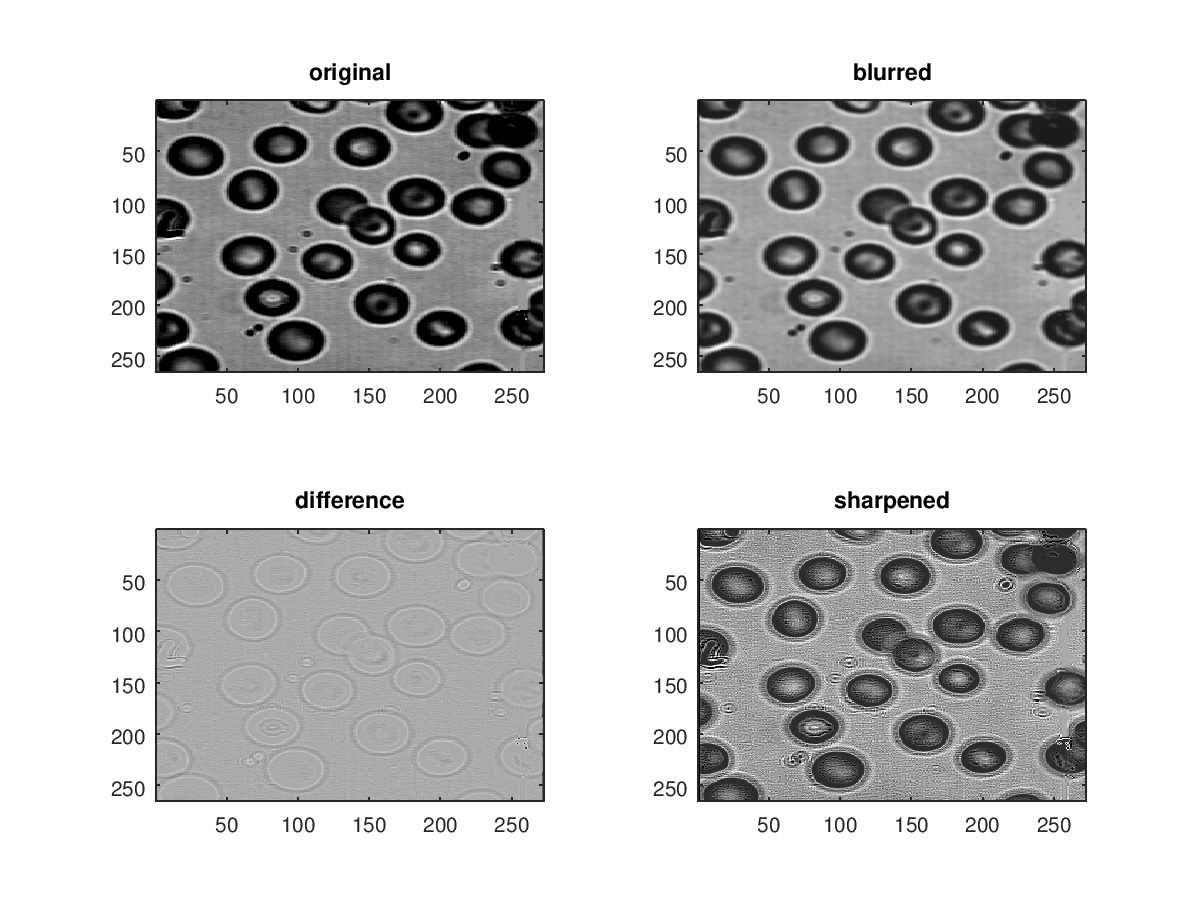
\includegraphics[width=0.75\textwidth]{sharpen}
                        \captionof{figure}{Slika {\it blood1.tif} u svim koracima postupka izoštravanja. Razlika se vidi na rubovima koji su izoštreni postupkom.}
                    \end{minipage}
                \item
                    \begin{minipage}{\linewidth}
                        \centering
                        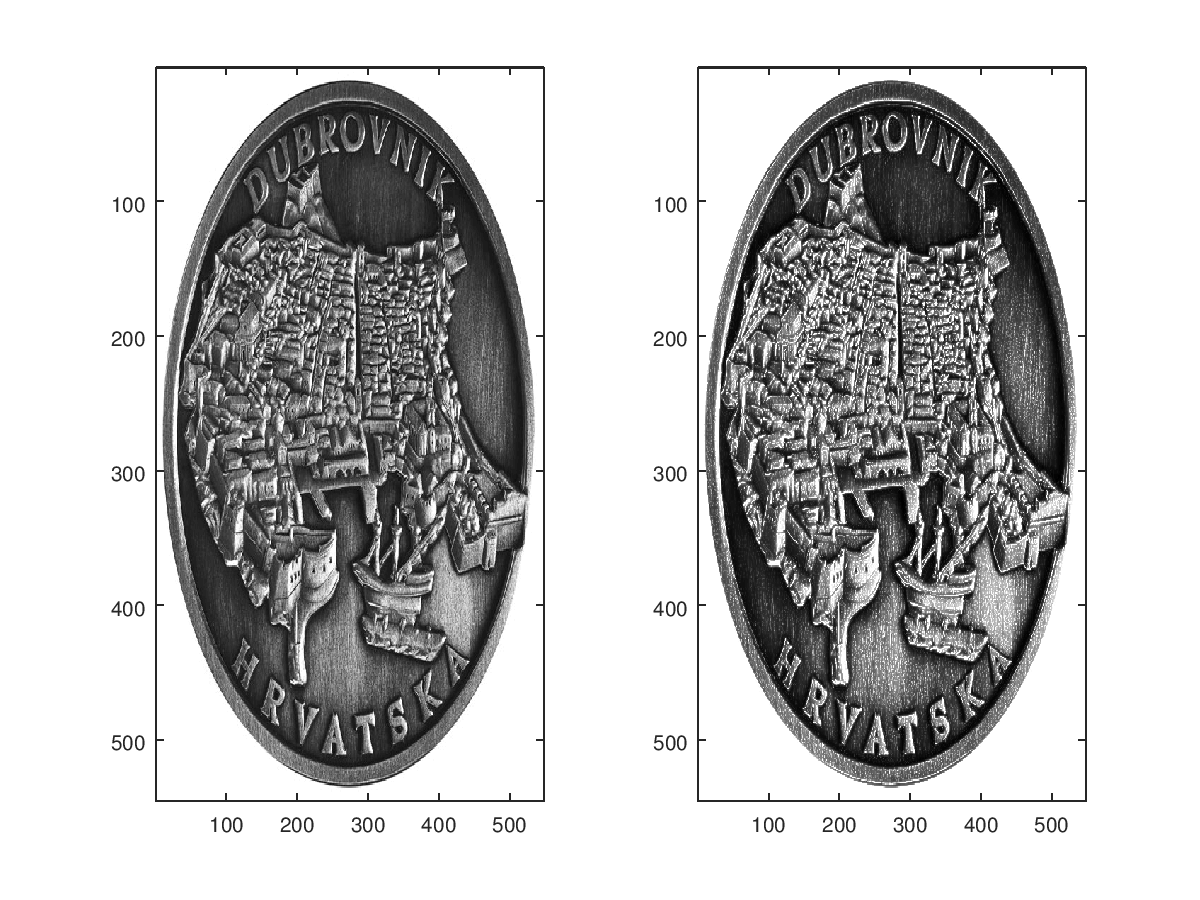
\includegraphics[width=0.75\textwidth]{medalja_blur}
                        \captionof{figure}{Slika {\it medalja\_dubrovnik.png} izoštrena postupkom oduzimanja zamućene slike.}
                    \end{minipage}
                \item
                    \begin{minipage}{\linewidth}
                        \centering
                        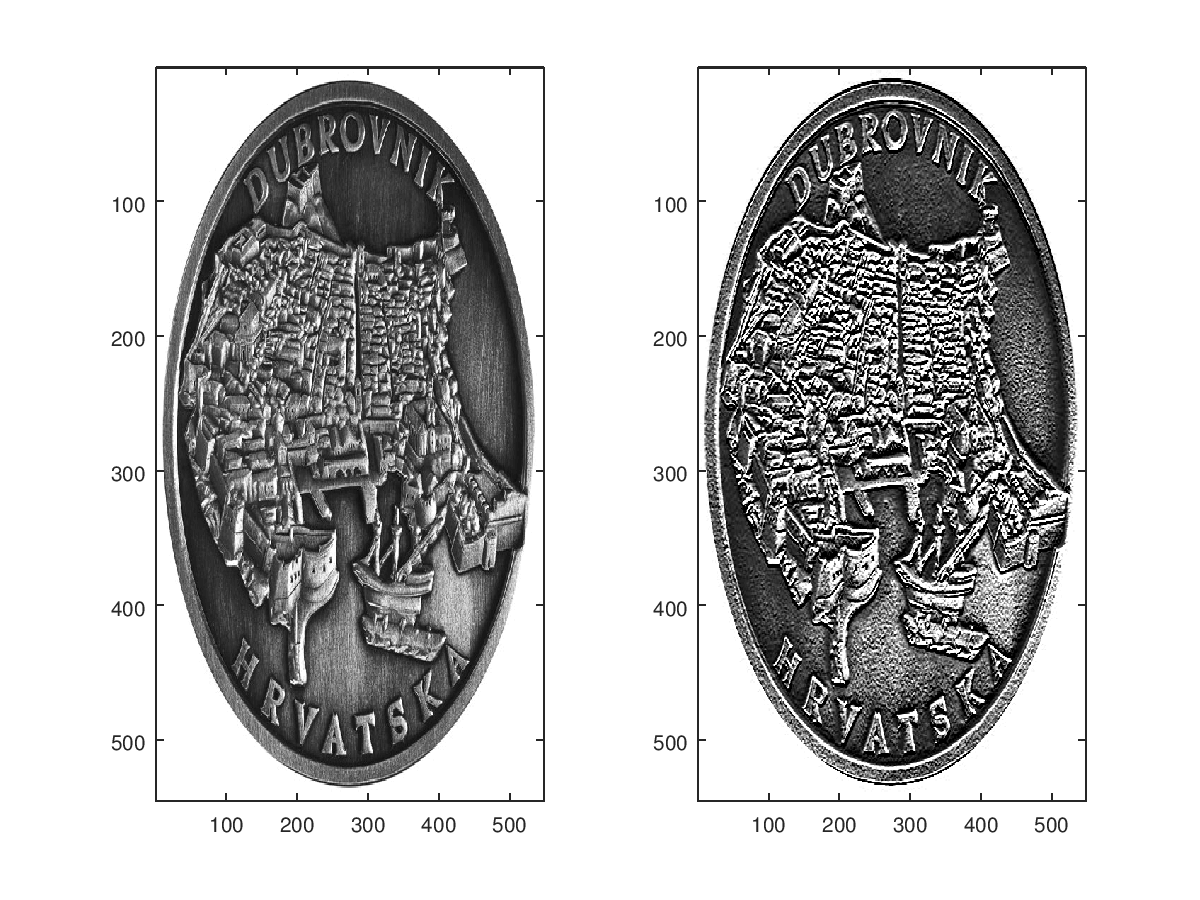
\includegraphics[width=0.75\textwidth]{medalja_sobel}
                        \captionof{figure}{Slika {\it medalja\_dubrovnik.png} izoštrena postupkom dodavanja procjene prve derivacije. Ovim postupkom su posebno istaknute visokofrekvencijske komponente.}
                    \end{minipage}
                \item
                    \begin{minipage}{\linewidth}
                        \centering
                        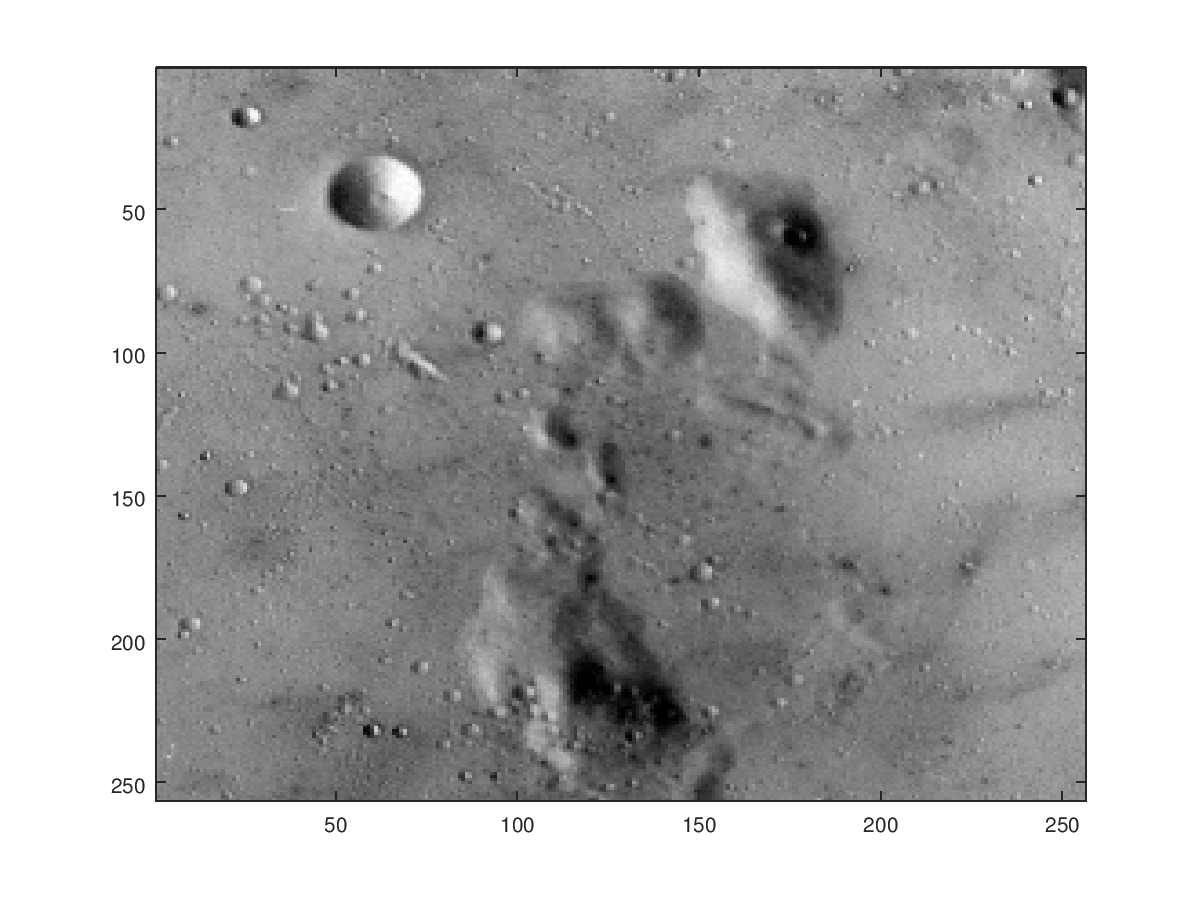
\includegraphics[width=0.75\textwidth]{moon}
                        \captionof{figure}{Originalna slika {\it 5.1.09.tiff}}
                    \end{minipage}
                    \begin{minipage}{\linewidth}
                        \centering
                        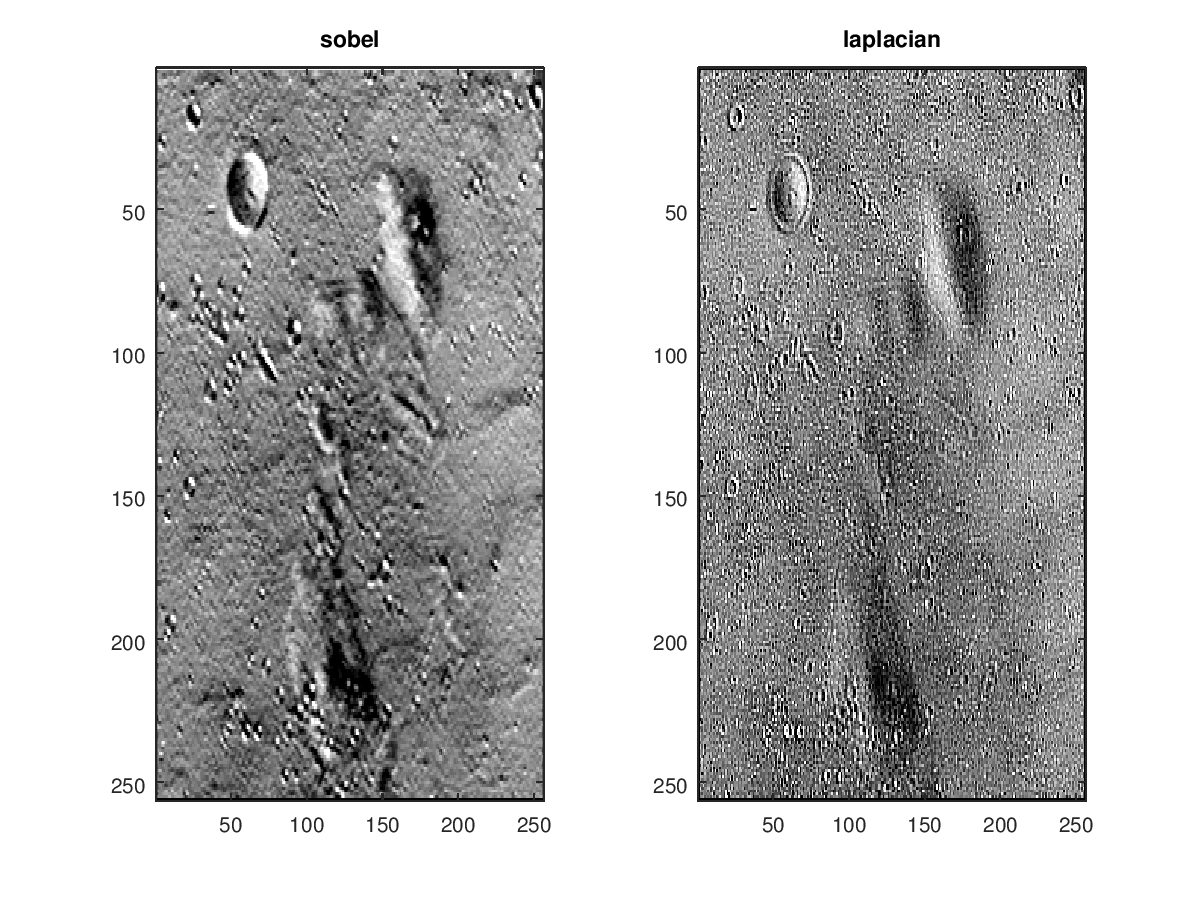
\includegraphics[width=0.75\textwidth]{moon_sharpen}
                        \captionof{figure}{Slika {\it 5.1.09.tiff} izoštrena Sobelovim i Laplaceovim operatorom. Laplaceov operator bolje izoštrava sitnije detalje na slici, a Sobel krupnije detalje.}
                    \end{minipage}
                \item
                    \begin{minipage}{\linewidth}
                        \centering
                        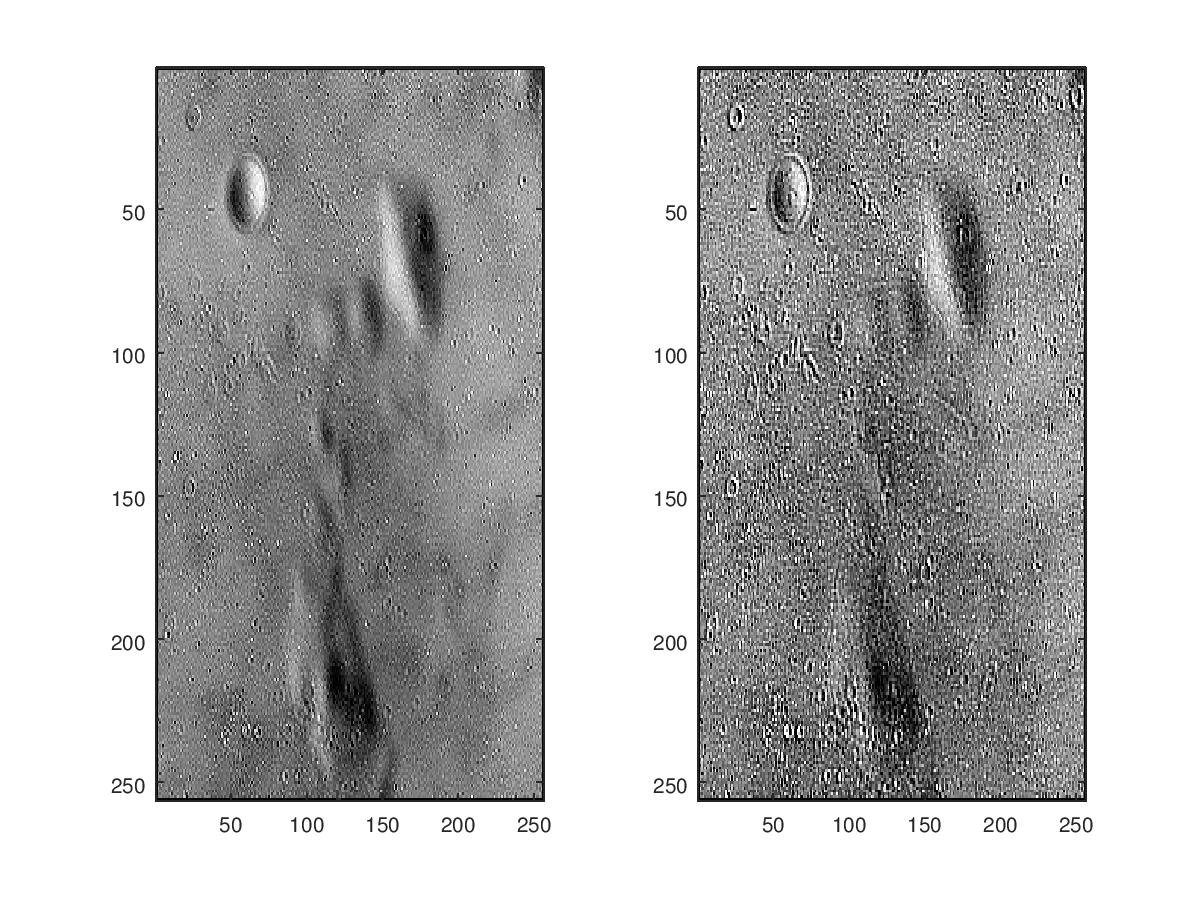
\includegraphics[width=0.75\textwidth]{moon_lap}
                        \captionof{figure}{Slika {\it 5.1.09.tiff} izoštrena Laplaceovim operatorom s različitim parametrima. {\tt lap2} uključuje i derivaciju po dijagonali pa je više rubova istaknuto.}
                    \end{minipage}
                \item
                    \begin{minipage}{\linewidth}
                        \centering
                        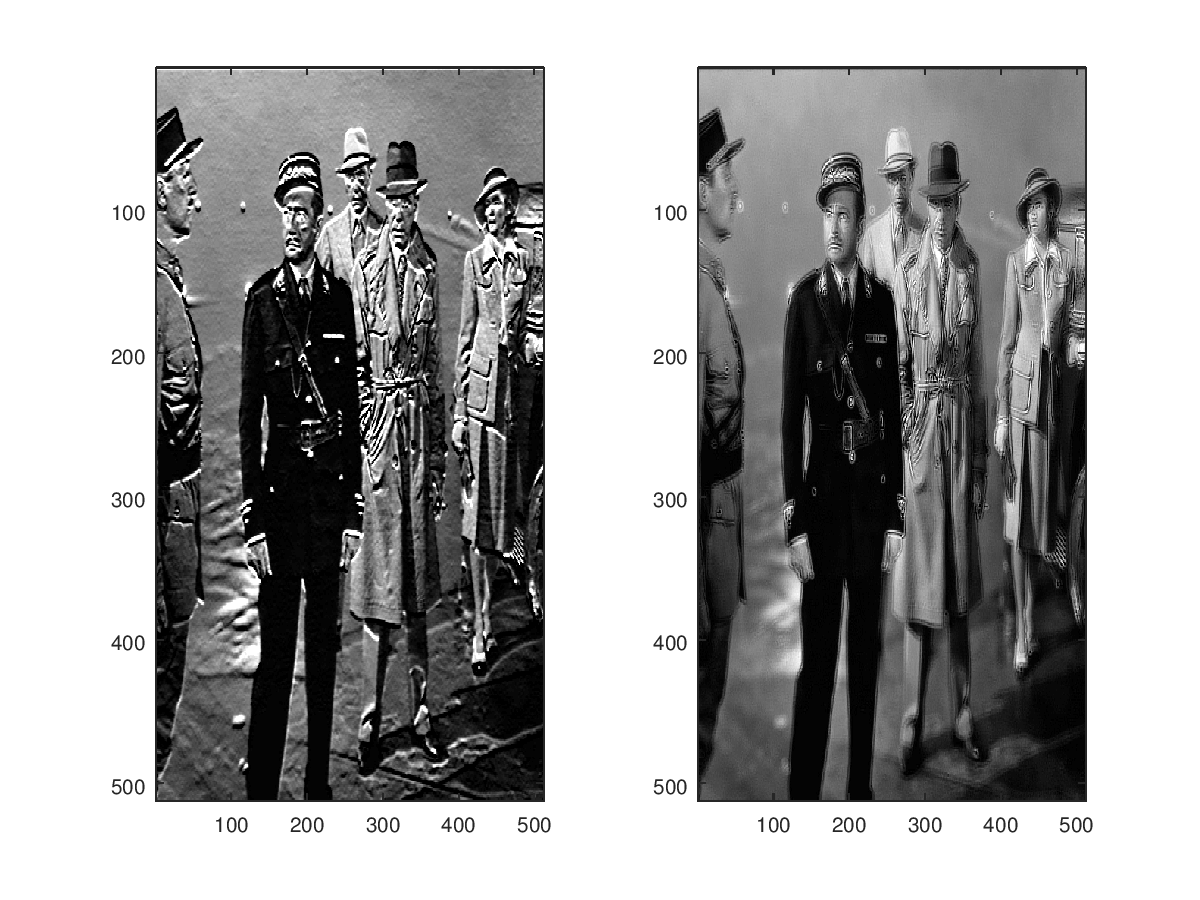
\includegraphics[width=0.75\textwidth]{casablanca_sharpen}
                        \captionof{figure}{Usporedba metoda dodavanja estimacije prve i druge derivacije na slici {\it casablanca.png}. Najveća je razlika što Laplaceov operator može više isticati šum koji je na slici.}
                    \end{minipage}    
            \end{enumerate}
    \end{document}

